\section{System Design}

% Slide 10
\begin{frame}
\frametitle{Functional Decomposition}

\begin{tabular}{l | l}
\toprule
\textbf{Component} & \textbf{Function} \\
\midrule
Honeypot Plugin Framework & Core, extensible interfaces \\
Default Plugin Set & Client-specific functionality \\
Automated Deployment System & Flexible rollouts/updates \\
Device & Components installed on device(s) \\
\bottomrule
\end{tabular}

\end{frame}

% Slide 11
\begin{frame}
\frametitle{Detailed Design: Honeypot Framework}

\begin{figure}
\centering
\caption{Plugin Framework Architecture}
{\scalefont{0.70}
\scalebox{0.7}{% Graphic for TeX using PGF
% Title: /home/nskinkel/plugins.dia
% Creator: Dia v0.97.3
% CreationDate: Sun Dec  6 18:02:21 2015
% For: nskinkel
% \usepackage{tikz}
% The following commands are not supported in PSTricks at present
% We define them conditionally, so when they are implemented,
% this pgf file will use them.
\ifx\du\undefined
  \newlength{\du}
\fi
\setlength{\du}{15\unitlength}
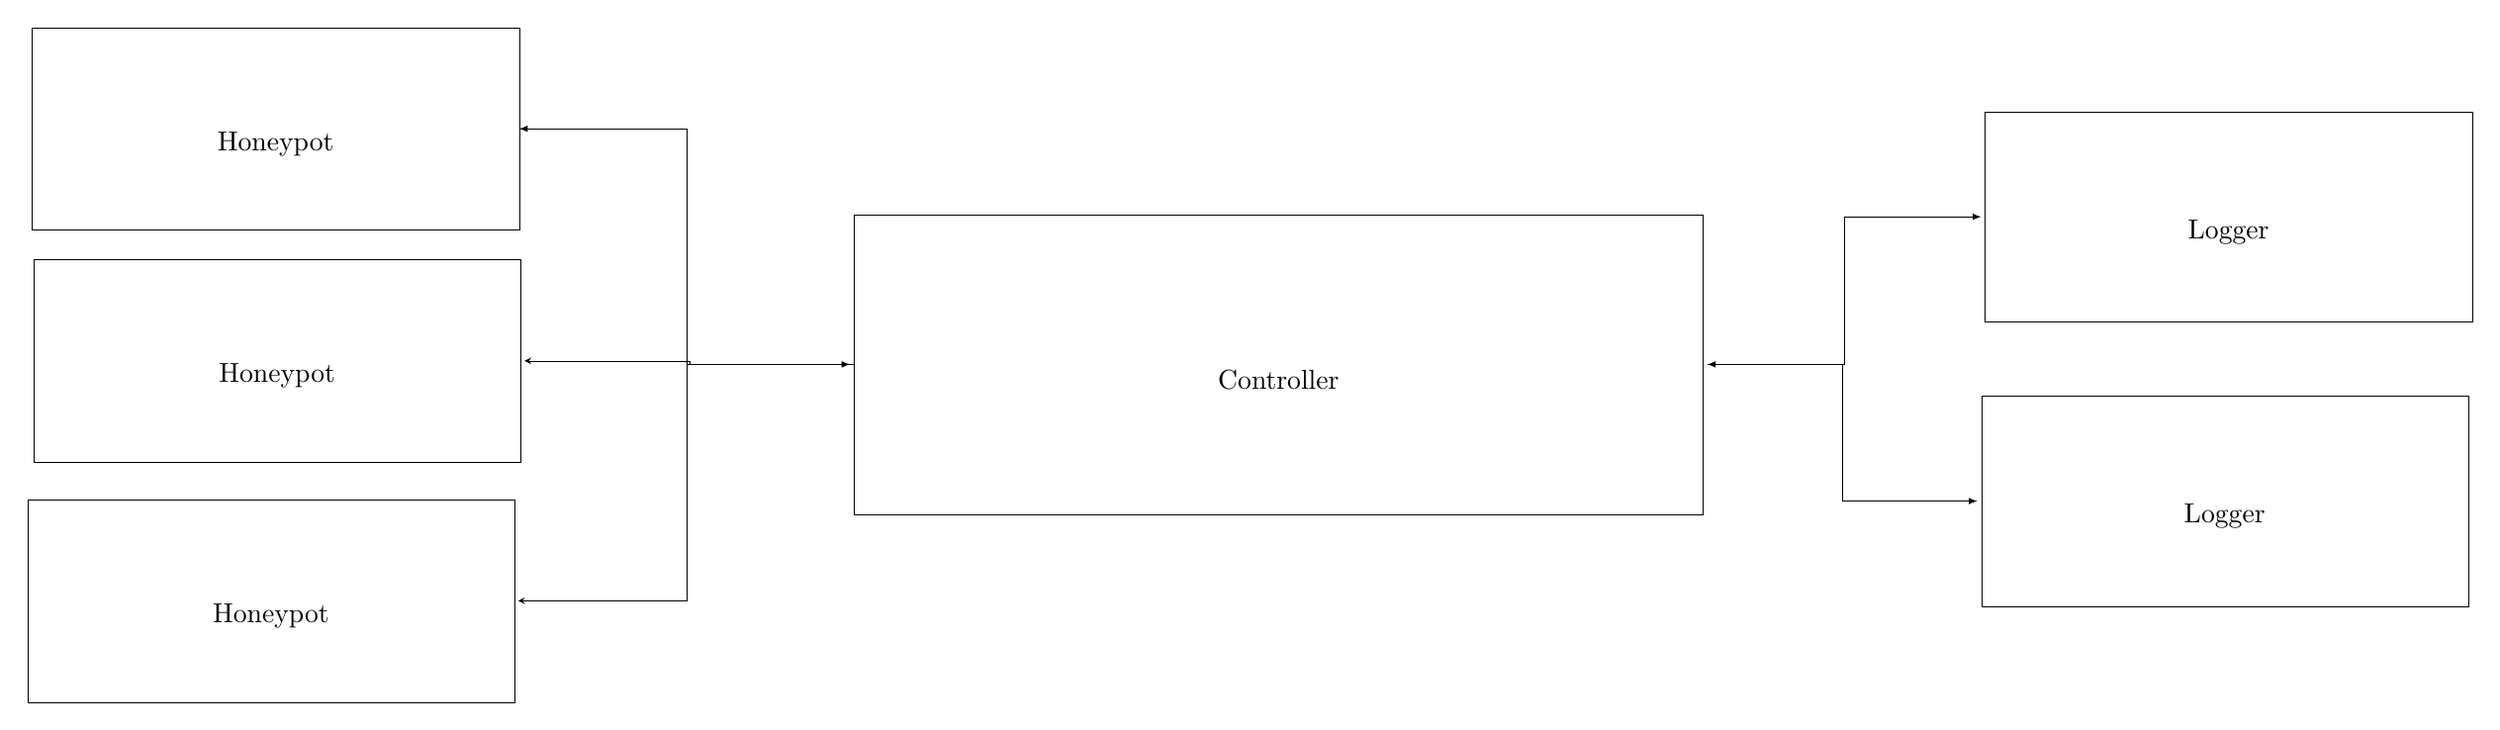
\begin{tikzpicture}
\pgftransformxscale{1.000000}
\pgftransformyscale{-1.000000}
\definecolor{dialinecolor}{rgb}{0.000000, 0.000000, 0.000000}
\pgfsetstrokecolor{dialinecolor}
\definecolor{dialinecolor}{rgb}{1.000000, 1.000000, 1.000000}
\pgfsetfillcolor{dialinecolor}
\definecolor{dialinecolor}{rgb}{1.000000, 1.000000, 1.000000}
\pgfsetfillcolor{dialinecolor}
\fill (6.250000\du,0.500000\du)--(6.250000\du,3.100000\du)--(12.500000\du,3.100000\du)--(12.500000\du,0.500000\du)--cycle;
\pgfsetlinewidth{0.100000\du}
\pgfsetdash{}{0pt}
\pgfsetdash{}{0pt}
\pgfsetmiterjoin
\definecolor{dialinecolor}{rgb}{0.000000, 0.000000, 0.000000}
\pgfsetstrokecolor{dialinecolor}
\draw (6.250000\du,0.500000\du)--(6.250000\du,3.100000\du)--(12.500000\du,3.100000\du)--(12.500000\du,0.500000\du)--cycle;
% setfont left to latex
\definecolor{dialinecolor}{rgb}{0.000000, 0.000000, 0.000000}
\pgfsetstrokecolor{dialinecolor}
\node at (9.375000\du,1.995000\du){Honeypot};
\definecolor{dialinecolor}{rgb}{1.000000, 1.000000, 1.000000}
\pgfsetfillcolor{dialinecolor}
\fill (6.270000\du,3.480000\du)--(6.270000\du,6.080000\du)--(12.520000\du,6.080000\du)--(12.520000\du,3.480000\du)--cycle;
\pgfsetlinewidth{0.100000\du}
\pgfsetdash{}{0pt}
\pgfsetdash{}{0pt}
\pgfsetmiterjoin
\definecolor{dialinecolor}{rgb}{0.000000, 0.000000, 0.000000}
\pgfsetstrokecolor{dialinecolor}
\draw (6.270000\du,3.480000\du)--(6.270000\du,6.080000\du)--(12.520000\du,6.080000\du)--(12.520000\du,3.480000\du)--cycle;
% setfont left to latex
\definecolor{dialinecolor}{rgb}{0.000000, 0.000000, 0.000000}
\pgfsetstrokecolor{dialinecolor}
\node at (9.395000\du,4.975000\du){Honeypot};
\definecolor{dialinecolor}{rgb}{1.000000, 1.000000, 1.000000}
\pgfsetfillcolor{dialinecolor}
\fill (6.190000\du,6.560000\du)--(6.190000\du,9.160000\du)--(12.440000\du,9.160000\du)--(12.440000\du,6.560000\du)--cycle;
\pgfsetlinewidth{0.100000\du}
\pgfsetdash{}{0pt}
\pgfsetdash{}{0pt}
\pgfsetmiterjoin
\definecolor{dialinecolor}{rgb}{0.000000, 0.000000, 0.000000}
\pgfsetstrokecolor{dialinecolor}
\draw (6.190000\du,6.560000\du)--(6.190000\du,9.160000\du)--(12.440000\du,9.160000\du)--(12.440000\du,6.560000\du)--cycle;
% setfont left to latex
\definecolor{dialinecolor}{rgb}{0.000000, 0.000000, 0.000000}
\pgfsetstrokecolor{dialinecolor}
\node at (9.315000\du,8.055000\du){Honeypot};
\definecolor{dialinecolor}{rgb}{1.000000, 1.000000, 1.000000}
\pgfsetfillcolor{dialinecolor}
\fill (31.320000\du,1.580000\du)--(31.320000\du,4.280000\du)--(37.570000\du,4.280000\du)--(37.570000\du,1.580000\du)--cycle;
\pgfsetlinewidth{0.100000\du}
\pgfsetdash{}{0pt}
\pgfsetdash{}{0pt}
\pgfsetmiterjoin
\definecolor{dialinecolor}{rgb}{0.000000, 0.000000, 0.000000}
\pgfsetstrokecolor{dialinecolor}
\draw (31.320000\du,1.580000\du)--(31.320000\du,4.280000\du)--(37.570000\du,4.280000\du)--(37.570000\du,1.580000\du)--cycle;
% setfont left to latex
\definecolor{dialinecolor}{rgb}{0.000000, 0.000000, 0.000000}
\pgfsetstrokecolor{dialinecolor}
\node at (34.445000\du,3.125000\du){Logger};
\definecolor{dialinecolor}{rgb}{1.000000, 1.000000, 1.000000}
\pgfsetfillcolor{dialinecolor}
\fill (31.270000\du,5.230000\du)--(31.270000\du,7.930000\du)--(37.520000\du,7.930000\du)--(37.520000\du,5.230000\du)--cycle;
\pgfsetlinewidth{0.100000\du}
\pgfsetdash{}{0pt}
\pgfsetdash{}{0pt}
\pgfsetmiterjoin
\definecolor{dialinecolor}{rgb}{0.000000, 0.000000, 0.000000}
\pgfsetstrokecolor{dialinecolor}
\draw (31.270000\du,5.230000\du)--(31.270000\du,7.930000\du)--(37.520000\du,7.930000\du)--(37.520000\du,5.230000\du)--cycle;
% setfont left to latex
\definecolor{dialinecolor}{rgb}{0.000000, 0.000000, 0.000000}
\pgfsetstrokecolor{dialinecolor}
\node at (34.395000\du,6.775000\du){Logger};
\definecolor{dialinecolor}{rgb}{1.000000, 1.000000, 1.000000}
\pgfsetfillcolor{dialinecolor}
\fill (16.800000\du,2.900000\du)--(16.800000\du,6.750000\du)--(27.700000\du,6.750000\du)--(27.700000\du,2.900000\du)--cycle;
\pgfsetlinewidth{0.100000\du}
\pgfsetdash{}{0pt}
\pgfsetdash{}{0pt}
\pgfsetmiterjoin
\definecolor{dialinecolor}{rgb}{0.000000, 0.000000, 0.000000}
\pgfsetstrokecolor{dialinecolor}
\draw (16.800000\du,2.900000\du)--(16.800000\du,6.750000\du)--(27.700000\du,6.750000\du)--(27.700000\du,2.900000\du)--cycle;
% setfont left to latex
\definecolor{dialinecolor}{rgb}{0.000000, 0.000000, 0.000000}
\pgfsetstrokecolor{dialinecolor}
\node at (22.250000\du,5.020000\du){Controller};
\pgfsetlinewidth{0.100000\du}
\pgfsetdash{}{0pt}
\pgfsetdash{}{0pt}
\pgfsetmiterjoin
\pgfsetbuttcap
{
\definecolor{dialinecolor}{rgb}{0.000000, 0.000000, 0.000000}
\pgfsetfillcolor{dialinecolor}
% was here!!!
\pgfsetarrowsstart{latex}
{\pgfsetcornersarced{\pgfpoint{0.000000\du}{0.000000\du}}\definecolor{dialinecolor}{rgb}{0.000000, 0.000000, 0.000000}
\pgfsetstrokecolor{dialinecolor}
\draw (12.500000\du,1.800000\du)--(14.650000\du,1.800000\du)--(14.650000\du,4.825000\du)--(16.800000\du,4.825000\du);
}}
\pgfsetlinewidth{0.100000\du}
\pgfsetdash{}{0pt}
\pgfsetdash{}{0pt}
\pgfsetmiterjoin
\pgfsetbuttcap
{
\definecolor{dialinecolor}{rgb}{0.000000, 0.000000, 0.000000}
\pgfsetfillcolor{dialinecolor}
% was here!!!
\pgfsetarrowsstart{stealth}
{\pgfsetcornersarced{\pgfpoint{0.000000\du}{0.000000\du}}\definecolor{dialinecolor}{rgb}{0.000000, 0.000000, 0.000000}
\pgfsetstrokecolor{dialinecolor}
\draw (12.570388\du,4.780000\du)--(14.685194\du,4.780000\du)--(14.685194\du,4.825000\du)--(16.800000\du,4.825000\du);
}}
\pgfsetlinewidth{0.100000\du}
\pgfsetdash{}{0pt}
\pgfsetdash{}{0pt}
\pgfsetmiterjoin
\pgfsetbuttcap
{
\definecolor{dialinecolor}{rgb}{0.000000, 0.000000, 0.000000}
\pgfsetfillcolor{dialinecolor}
% was here!!!
\pgfsetarrowsstart{stealth}
\pgfsetarrowsend{latex}
{\pgfsetcornersarced{\pgfpoint{0.000000\du}{0.000000\du}}\definecolor{dialinecolor}{rgb}{0.000000, 0.000000, 0.000000}
\pgfsetstrokecolor{dialinecolor}
\draw (12.489169\du,7.860000\du)--(14.650000\du,7.860000\du)--(14.650000\du,4.825000\du)--(16.749927\du,4.825000\du);
}}
\pgfsetlinewidth{0.100000\du}
\pgfsetdash{}{0pt}
\pgfsetdash{}{0pt}
\pgfsetmiterjoin
\pgfsetbuttcap
{
\definecolor{dialinecolor}{rgb}{0.000000, 0.000000, 0.000000}
\pgfsetfillcolor{dialinecolor}
% was here!!!
\pgfsetarrowsend{latex}
{\pgfsetcornersarced{\pgfpoint{0.000000\du}{0.000000\du}}\definecolor{dialinecolor}{rgb}{0.000000, 0.000000, 0.000000}
\pgfsetstrokecolor{dialinecolor}
\draw (27.750336\du,4.825000\du)--(29.484974\du,4.825000\du)--(29.484974\du,6.580000\du)--(31.219612\du,6.580000\du);
}}
\pgfsetlinewidth{0.100000\du}
\pgfsetdash{}{0pt}
\pgfsetdash{}{0pt}
\pgfsetmiterjoin
\pgfsetbuttcap
{
\definecolor{dialinecolor}{rgb}{0.000000, 0.000000, 0.000000}
\pgfsetfillcolor{dialinecolor}
% was here!!!
\pgfsetarrowsstart{latex}
\pgfsetarrowsend{latex}
{\pgfsetcornersarced{\pgfpoint{0.000000\du}{0.000000\du}}\definecolor{dialinecolor}{rgb}{0.000000, 0.000000, 0.000000}
\pgfsetstrokecolor{dialinecolor}
\draw (27.750336\du,4.825000\du)--(29.509974\du,4.825000\du)--(29.509974\du,2.930000\du)--(31.269612\du,2.930000\du);
}}
\end{tikzpicture}
}
}
\end{figure}

\begin{table}
\centering
\small
\begin{tabularx}{\linewidth}{l l}
\textbf{Modular, Extensible} & \textbf{Secure by Design} \\
\midrule
2 plugin types: Honeypot \& Logger & Isolated, non-privileged processes \\
Communicate via lo unix socket RPC & Minimal protocol functionality \\
\end{tabularx}
\end{table}
\end{frame}

% Slide 12
\begin{frame}
\frametitle{Technology Platform}
\textbf{CanaKit Raspberry PI}
\begin{itemize}
\item Quad-Core 900 MHz Processor
\item 1GB Ram
\item Rasbian OS
\end{itemize}

\textbf{Software}
\begin{itemize}
\item Ansible (Provisioning)
\item Vagrant (Provisioned Testing)
\item Golang (Google Programming Language)
\end{itemize}


\end{frame}

% Slide 13
\begin{frame}

\frametitle{Test Plan}
\textbf{GoLang}

Integration testing can be completed by combining multiple unit tests into a larger framework with the "testing" package. 
What about multiple configurations or platforms though?\\~\\

\textbf {Vagrant} allows for easy replication of test environments through virtual machines. This provides a method for plugin end-end testing for any device setup. \\~\\

Vagrant allows for \textbf{Provisioning}. This means that a newly created VM can be give startup tasks that will run as an automated script.

\end{frame}

% Slide 13.1
\begin{frame}[fragile]
\frametitle{Test Plan Continued}
\begin{itemize} % Elaborate on each item
	\item Time complexity analysis
	\item Code output verification
	\end{itemize}

\begin{example}[Benchmark Code] % Explain Code & Elaborate on output testing
\begin{verbatim}
	func BenchmarkSplunk (b *testing.B){
		m := map[string]string{"username":"user","password":"pass"}
		http:=Http{Method:"POST",Path:"index.html",Parameters:m}
		ev := Event{...,Http: &http}
		for i := 0 ; i< b.N; i++{
			ev.Send();
		}
	}
\end{verbatim}
\end{example}
	\textbf{Output}
	BenchmarkSplunk    10000000    282 ns/op


\end{frame}

% Slide 14
\begin{frame}
\frametitle{Prototype Implementation}

\begin{table}
\centering
\small
\begin{tabularx}{\linewidth}{c X X}
\toprule
\textbf{Component} & \textbf{Code} & \textbf{Status} \\
\midrule
Default Plugin Set & \begin{itemize}[leftmargin=-0.3mm,after=\vspace{-\baselineskip},noitemsep,nolistsep]
                         \item[] \href{https://github.com/Senior-Design-May1601/webauth}{HTTP}
                         \item[] \href{https://github.com/Senior-Design-May1601/webauth}{HTTPS}
                         \item[] \href{https://github.com/Senior-Design-May1601/fssh}{SSH}
                         \item[] \href{https://github.com/Senior-Design-May1601/Splunk}{Splunk Logger}
                     \end{itemize} &
                    \begin{itemize}[leftmargin=-0.3mm,after=\vspace{-\baselineskip},noitemsep,nolistsep]
                         \item[] \textcolor{ao(english)}{Done}
                         \item[] \textcolor{ao(english)}{Done}
                         \item[] \textcolor{ao(english)}{Done}
                         \item[] \textcolor{ao(english)}{Done}
                     \end{itemize} \\ \hline
Automatic Deployment and Updates & \href{https://github.com/Senior-Design-May1601/config}{Ansible playbooks} & \textcolor{ao(english)}{Done} \\ \hline
Plugin Core & \href{https://github.com/Senior-Design-May1601/projectmain}{Framework} & Work-in-progress \\ \hline
Physical Install & N/A & \textcolor{bostonuniversityred}{TODO} \\ \hline
Testing & N/A & \textcolor{bostonuniversityred}{TODO} \\
\bottomrule
\end{tabularx}
\end{table}
\end{frame}
